\documentclass{6006}

% \documentclass[12pt, tikz, margin=3mm]{standalone}
\usepackage{enumerate}
\usepackage{color}
\usepackage{xcolor}
\usepackage{listings}
\usepackage{mathtools}
\usepackage{graphicx}
\graphicspath{ {./} }
\usepackage{pgfplots}
\lstset{language=Python,keywordstyle={\bfseries \color{blue}}}
\definecolor{mygreen}{rgb}{0,0.6,0}
\definecolor{mygray}{rgb}{0.5,0.5,0.5}
\definecolor{mymauve}{rgb}{0.58,0,0.82}
\definecolor{codegreen}{rgb}{0,0.6,0}
\definecolor{codegray}{rgb}{0.5,0.5,0.5}
\definecolor{codepurple}{rgb}{0.58,0,0.82} 
\definecolor{backcolour}{rgb}{0.95,0.95,0.92}
\lstset{ %
  backgroundcolor=\color{white},   % choose the background color
  basicstyle=\footnotesize,        % size of fonts used for the code
  breaklines=true,                 % automatic line breaking only at whitespace
  captionpos=b,                    % sets the caption-position to bottom
  commentstyle=\color{mygreen},    % comment style
  escapeinside={\%*}{*)},          % if you want to add LaTeX within your code
  keywordstyle=\color{blue},       % keyword style
  stringstyle=\color{mymauve},     % string literal style
  backgroundcolor=\color{backcolour},   
    commentstyle=\color{codegreen},
    keywordstyle=\color{magenta},
    numberstyle=\tiny\color{codegray},
    stringstyle=\color{codepurple},
    basicstyle=\ttfamily\footnotesize,
    breakatwhitespace=false,         
    breaklines=true,                 
    captionpos=b,                    
    keepspaces=true,                 
    numbers=left,                     
    numbersep=5pt,                  
    showspaces=false,                
    showstringspaces=false,
    showtabs=false,                  
    tabsize=2
}

\author{Sanjay Seshan and Bill Wang}
\collab{None}
\problem{None}
\usetikzlibrary{arrows.meta, automata, positioning, quotes}

\begin{document}

Let’s consider the following maze.
We will solve this using two approaches:
\begin{enumerate}[(a)]
        \item Solve this using a right hand rule method/follow the wall
        \item Solve this by considering all outgoing paths at each branch one at a time (DFS – depth first search)
\end{enumerate}
\includegraphics*[width=5cm]{figures/maze_bfs_lg.png}
\includegraphics*[width=5cm]{figures/maze_bfs_lg.png}

What patterns do you notice? Does this give you the ``best'' path? Is there a better path?

Let's try to find the best path below.

\includegraphics*[width=5cm]{figures/maze_bfs_lg.png}

How do you decide which path to take at each intersection? How does it scale to many branches? We are developing the Breath First Search (BFS).


\newpage

Let's consider an expanded problem -- Train routes in Europe
What is the shortest path from London to Metz?
In terms of stops? In terms of distance? 

Assume all trains are the same speed and there is no time lost between stops. 

\includegraphics*[width=8cm]{figures/london_trains.png}

Are all stops evenly spaced? What is ``shortest'' here?

Consider a reduced representation -- what is the shortest path from E to D? Let the number on the arrow be the distance from each node or city. The direction of the arrow maps the direction of travel permitted. What pattern do you see? 

    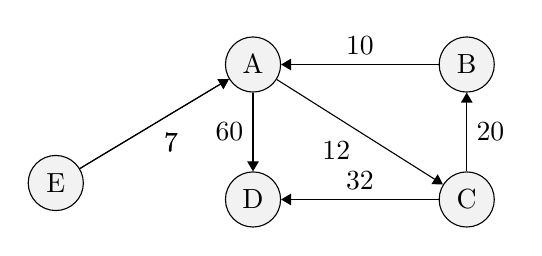
\begin{tikzpicture}[
node distance = 10mm and 20mm,
every state/.append style = {inner sep=0pt, fill=gray!10,
                             minimum size=7mm},
every edge/.style = {draw, -Triangle, bend angle=15},
                auto=right,
                        ]
\node (s1) [state]         {E};
\node (s2) [state, above right=of s1]   {A};
\node (s3) [state, below=of s2]         {D};
\node (s4) [state,  right=of s3]   {C};
\node (s5) [state, above =of s4]   {B};
\draw   (s1) edge ["7"]             (s2)
(s1) edge ["7"]             (s2)
(s2) edge ["12"]             (s4)
(s2) edge ["60"]             (s3)
(s4) edge ["20"]             (s5)
(s5) edge ["10"]             (s2)
(s4) edge ["32"]             (s3);
   \end{tikzpicture}

   This is called Dijkstra's algorithm.

   Can we represent the above map, or a maze, like this?

 \newpage


\begin{lstlisting}
def run_dfs(pixels,curr,visited):
    for dr, dc in [(___,___),(___,___),(___,___),(___,___)]:
        visited.add(curr)
        new = curr[0] + dr, curr[1] + dc
        if new[0] < rdim and new[1] < cdim and new[0] >=0 and new[1] >=0:
            if pixels[new[0],new[1]] == ______:
                return ______,______
            elif pixels[new[0],new[1]] == ______:
                if new not in visited:
                    res = _________________________
                    if res is not None:
                        return (curr,)+______
                    else:
                        _________________________
    return None
pos = run_dfs(pixels,(0,1),set())
\end{lstlisting}
\begin{lstlisting}  
def run_bfs(pixels,rdim,cdim):
    Q = [((0,1),)]
    while Q != []:
        path = Q.pop(___)
        curr = path[-1]
        for dr, dc in [(___,___),(___,___),(___,___),(___,___)]:
            new = curr[0] + dr, curr[1] + dc
            if  new[0] < rdim and new[1]<cdim and new[0]>=0 and new[1]>=0:
                if pixels[new[0],new[1]] == ______:
                    return _________________________
                elif pixels[new[0],new[1]] == ______:
                    if _________________:
                        new_path = path+_________________
                        _________________________
pos = run_bfs(pixels,rdim,cdim)
\end{lstlisting}
\begin{lstlisting}
def run_dijkstra(nodes):
    Q = [((nodes[0],),0)]
    while Q != []:
        imin = 0
        vmin = None
        for i in range(len(Q)):
            if vmin is None or Q[i][1] < vmin:
                vmin = Q[i][1]
                imin = i
        path, dist = Q.pop(_________)
        curr = path[-1]
        for child, next_dist in curr.get_children():
            if child == nodes[-1]:
                return _________________________
            elif child not in path:
                new_path = _________________________
                Q.append(_________________________)
pos = run_dijkstra(mini)
\end{lstlisting}

% \begin{lstlisting}
% def run_dfs(pixels,curr,visited):
%     for dr, dc in [(1,0),(-1,0),(0,1),(0,-1)]:
%         visited.add(curr)
%         new = curr[0] + dr, curr[1] + dc
%         if new[0] < rdim and new[1] < cdim and new[0] >=0 and new[1] >=0:
%             if pixels[new[0],new[1]] == red:
%                 return (curr,new)
%             elif pixels[new[0],new[1]] == white:
%                 if new not in visited:
%                     res = run_dfs(pixels, new, visited)
%                     if res is not None:
%                         return (curr,)+res
%                     else:
%                         visited.remove(curr)
%     return None
% pos = run_dfs(pixels,(0,1),set())
% \end{lstlisting}
% \begin{lstlisting}  
% def run_bfs(pixels,rdim, cdim):
%     Q = [((0,1),)]
%     while Q != []:
%     path = Q.pop(0)
%     curr = path[-1]
%     for dr, dc in [(1,0),(0,1),(-1,0),(0,-1)]:
%         new = curr[0] + dr, curr[1] + dc
%         if  new[0] < rdim and new[1] < cdim and new[0] >=0 and new[1] >=0:
%         if pixels[new[0],new[1]] == red:
%             return path+(new,)
%         elif pixels[new[0],new[1]] == white:
%             if new not in path:
%                 new_path = path+(new,)
%                 Q.append(new_path)
% \end{lstlisting}
% \begin{lstlisting}
% def run_dijkstra(nodes):
%     Q = [((nodes[0],),0)]
%     while Q != []:
%         imin = 0
%         vmin = None
%         for i in range(len(Q)):
%             if vmin is None or Q[i][1] < vmin:
%                 vmin = Q[i][1]
%                 imin = i
%         path, dist = Q.pop(imin)
%         curr = path[-1]
%         for child, next_dist in curr.get_children():
%             if child == nodes[-1]:
%                 return path+(child,)
%             elif child not in path:
%                 new_path = path+(child,)
%                 Q.append((new_path,dist+next_dist))
% \end{lstlisting}
\newpage

\textbf{References:}

\begin{lstlisting}
class Node(object):
    def __init__(self, name):
        self.children = []
        self.name = name
    
    def add_connection(self, child, distance):
        self.children.append((child,distance))

    def get_children(self):
        return self.children
    
    def __repr__(self):
        return self.name

E = Node("E")
A = Node("A")
D = Node("D")
C = Node("C")
B = Node("B")
mini = [E,A,C,B,D]
E.add_connection(A,7)
D.add_connection(A,60)
A.add_connection(C,12)
C.add_connection(B,20)
B.add_connection(A,10)
C.add_connection(D,32)
\end{lstlisting}

\begin{lstlisting}
from PIL import Image

im = Image.open("maze_bfs.png")

pixels = im.load()

rdim, cdim = im.size

red = (255,0,0, 255)
blue = (0,0,255, 255)
white = (255,255,255, 255)
black = (0,0,0, 255)
\end{lstlisting}
\end{document}

